\noindent
\textbf{Thermodynamics:
\ifthenelse{\equal{\solutions}{true}}{Examples}{Homework} for chapter 4.}\\

\begin{enumerate}

\item One mole of nitrogen gas is allowed to expand from 0.5 to 10 L (reversible and isothermal process at 300 K). Calculate the change in molar entropy using (a) the ideal
gas law and (b) the van der Waals equation with $a = 1.408$ atm L$^2$ mol$^{-2}$, $b = 0.03913$ L mol$^{-1}$.

\ifthenelse{\equal{\solutions}{true}}{% Problem 4/1 solution
\noindent
\underline{Solution:}\\

\noindent
The operations are: $E$, $C_2$, $C_2'$, $C_2''$, $S_4$, $S_4^3$, $\sigma_v$, $\sigma_v'$.\\
The $C_2$ axis is along C = C = C. The $C_2'$ and $C_2''$ axes are perpendicular to the $C_2$ axis
and are locate long the plane of the paper and perpendicular to the plane.\\

\hrule\vspace{0.5cm}



}{}

\item Derive the relation for $\bar{C}_P - \bar{C}_V$ for a gas that follows the van der Waals equation.

\ifthenelse{\equal{\solutions}{true}}{% Problem 4/2 solution
\noindent
\underline{Solution:}\\

\noindent
The group is Abelian, which means that the order of multiplication does not matter, which simplifies the problem. The products can be worked out as follows:\\

\noindent
Multiplication by $OE$ (the identity operation) always yields $O$ as the result (where $O$ is one of the symmetry operations in $C_{2v}$).
Also operations such as $OO$ give $E$ (rotation and reflection). The only remaining operations are between $C_2$, $\sigma_v(xz)$ and $\sigma_v'(yz)$.
The molecule is taken to reside in $yz$ plane. 

\noindent
Let's consider $C_2\sigma_v$ as an example. To visualize what is happening, think about NO$_2$ molecul and place $p_x$ atomic orbitals on the oxygen
atoms. Note that the $x$ direction is out of the paper plane. $C_2$ will exchange the two oxygens and at the same time flip the $p_x$ orbitals around.
Then $\sigma_v$ reflection just exchanges the oxygens again but without flipping the $p_x$ orbitals. The net effect was to get flip the $p_x$ orbitals.
This same effect may be obtained by $\sigma_v'$ operation and therefore $C_2\sigma_v = \sigma_v'$. The same method can be used to go over all
the remaineng elements in the product table.\\

\hrule\vspace{0.5cm}



}{}

\item Estimate the change in molar entropy of liquid benzene at 25 $^\circ$C and atmospheric pressure when the pressure is raised to 1000 bar? The coefficient of thermal expansion $\alpha$ is 1.237 $\times$ 10$^{-3}$ K$^{-1}$, the density is 0.879 g cm$^{-3}$, and the molar mass is 78.11 g mol$^{-1}$.

\ifthenelse{\equal{\solutions}{true}}{% Problem 4/3 solution
\noindent
\underline{Solution:}\\

\noindent
In a) and b) only $C_s$ symmetry element. The point group is $C_s$.\\
In c) the symmetry elements are: $C_\infty$ axis, $\infty$ number of perpendicular $C_2$ axes and $\sigma_v$ planes and
$\sigma_h$ plane. The poing group is $D_{\infty h}$.\\
In d) the symmetry elements are: $C_\infty$ axis and $\infty$ many $\sigma_v$ planes. The point group is $C_{\infty v}$.\\
In both e) and f) the symmetry elements are: $C_2$ axis and two $\sigma_v$ planes. The point group is $C_{2v}$.\\

\hrule\vspace{0.5cm}



}{}

\item Derive the expression for $\left(\partial U / \partial V\right)_T$ (the internal pressure) for a gas following the virial equation with $Z = 1 + B / V$. Consider only $PV$-work and a reversible process. Note that $B = B(T)$ (i.e. it depends on temperature).

\ifthenelse{\equal{\solutions}{true}}{% Problem 4/4 solution
\noindent
\underline{Solution:}\\

Recall the first law of thermodynamics: $dU = dq + dw$. For $PV$-work $dw = -PdV$ and by the second law: $dq = TdS$. Thus: $dU = TdS - PdV$ and dividing both sides by $dV$ and imposing constant temperature:

$$\left(\frac{\partial U}{\partial V}\right)_T = T\left(\frac{\partial S}{\partial V}\right)_T - P = T\left(\frac{\partial P}{\partial T}\right)_{\bar{V}} - P$$

The equation of state gives:

$$\frac{P\bar{V}}{RT} = 1 + \frac{B}{V}\Rightarrow P = \frac{RT}{\bar{V}} + \frac{BRT}{\bar{V}^2}$$

Furthermore, differentiation of $P$ with respect to $T$ gives:

$$\left(\frac{\partial P}{\partial T}\right)_{\bar{V}} = \frac{R}{\bar{V}} + \frac{BR}{\bar{V}^2} + \left(\frac{\partial B}{\partial T}\right)\frac{RT}{\bar{V}^2}$$

By inserting these results into the expression derived above:

$$\left(\frac{\partial U}{\partial V}\right)_T = T\left(\frac{R}{\bar{V}} + \frac{BR}{\bar{V}^2} + \left(\frac{\partial B}{\partial T}\right)_{\bar{V}}\frac{RT}{\bar{V}^2}\right) - \frac{RT}{\bar{V}} - \frac{BRT}{\bar{V}^2} = \left(\frac{\partial B}{\partial T}\right)_{\bar{V}}\frac{RT^2}{\bar{V}^2}$$

\hrule\vspace{0.5cm}
}{}

\item Consider the process of freezing water at $-10$ $^\circ$C for which the enthalpy change is $-5619$ J mol$^{-1}$ and entropy change is $-20.54$ J K$^{-1}$ mol$^{-1}$. What is the Gibbs energy of freezing water at constant temperature of $-10$ $^\circ$C?

\ifthenelse{\equal{\solutions}{true}}{% Problem 5/4 solution
\noindent
\underline{Solution:}\\

The Gibbs energy can be written in terms of enthalpy: $G = H - TS$. At constant temperature we have: $\Delta G = \Delta H - T\Delta S = -5619 \textnormal{ J mol}^{-1} - (263.15 \textnormal{ K})(-20.54\textnormal{ J K}^{-1}\textnormal{ mol}^{-1}) = -213.9\textnormal{ J mol}^{-1}$.

\hrule\vspace{0.5cm}
}{}

\item (a) Integrate the Gibbs-Helmholtz to obtain an expression for $\Delta G_2$ at temperature $T_2$ in terms of $\Delta G_1$ at $T_1$, assuming that $\Delta H$ is independent of temperature. (b) Obtain an expression for $\Delta G_2$ using a more accurate approximation that $\Delta H = \Delta H_1 + (T - T_1)\Delta C_P$, where $T_1$ is an arbitrary reference temperature. Assume that $\Delta C_P$ is temperature independent. Hint: Integrate one side with respect to variable $\Delta G / T$ and the other with respect to $T$.

\ifthenelse{\equal{\solutions}{true}}{% Problem 4/6 solution
\noindent
\underline{Solution:}\\

\noindent
The orbitals $S_1$ and $S_2$ can be visualized as shown below (the first figure).
\begin{figure}[h]
\centering
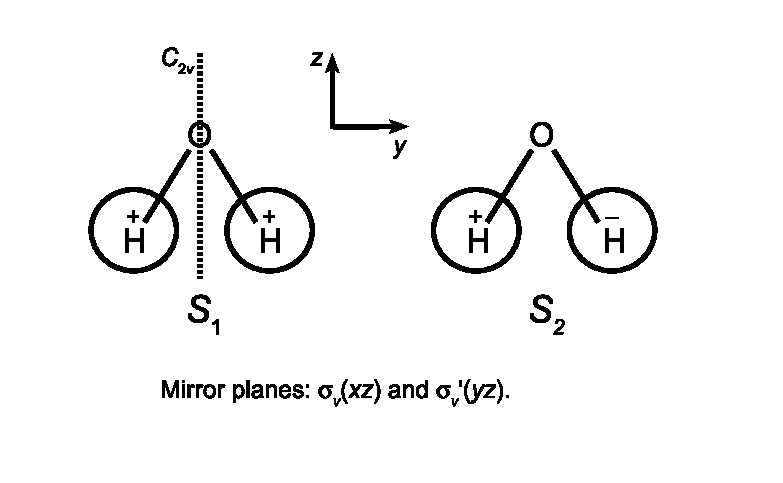
\includegraphics[scale=0.45]{watermo}
\caption{Visualization of $S_1$ and $S_2$ orbitals.}
\end{figure}
From this we can see that $S_1$ corresponds to $A_1$ (all operations give 1) and $S_2$ to $B_2$ (characters 1 $-1$ $-1$ 1).
The symmetry labels for the orbitals are therefore $a_1$ and $b_2$, respectively. The oxygen atom orbitals are shown in the second figure below.
\begin{figure}[h]
\centering
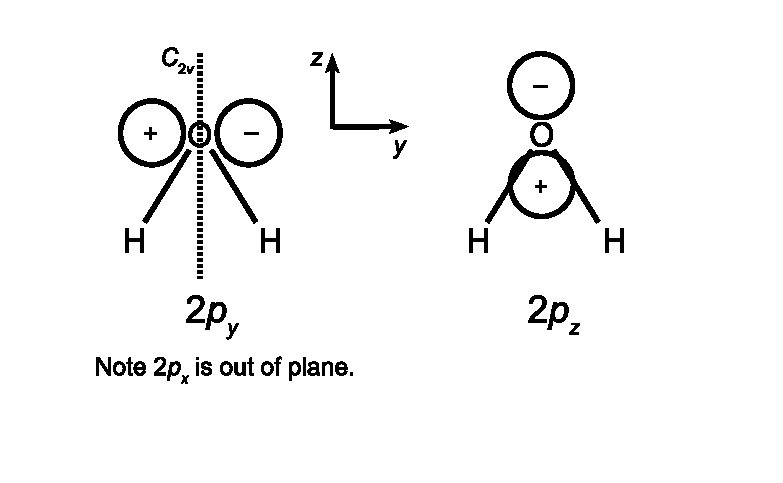
\includegraphics[scale=0.45]{watermo2}
\caption{Visualization of oxygen atom orbitals.}
\end{figure}
The $2s$ O orbital is clearly $A_1$ (totally symmetric). According to the above picture, $2p_z$ is also $A_1$. $p_y$ appears to
be $B_2$ and $p_x$ $B_1$. To find possible non-zero overlap integral value ($S$), we have to find pairs that produce $A_1$ when multiplied. Essentially, this says
that they must have the same symmetry. Thus $S_1$ can combine with $2s$ and $2p_z$ and $S_2$ with $2p_y$.\\

\hrule\vspace{0.5cm}



}{}

\item An ideal gas is allowed to expand reversibly and isothermally (25 $^\circ$C) from a pressure of 1 bar to a pressure of 0.1 bar. (a) What is the change in molar Gibbs energy? (b) What would be the change in molar Gibbs energy if the process occurred irreversibly?

\ifthenelse{\equal{\solutions}{true}}{% Problem 7/4 solution
\noindent
\underline{Solution:}\\

\begin{itemize}
\item[a)] Use the following equation (see lecture notes):

$$\Delta G_2 = RT\ln\left(\frac{P_2}{P_1}\right) = (8.314\textnormal{ J K}^{-1}\textnormal{ mol}^{-1})\times (298.15\textnormal{ K})\times\ln\left(\frac{0.1\textnormal{ bar}}{1\textnormal{ bar}}\right)$$
$$ = -5.708\textnormal{ kJ mol}^{-1}$$

\item[b)] Gibbs energy is a state function and depends only on the endpoints. Thus the answer is the same as in a).

\end{itemize}

\hrule\vspace{0.5cm}
}{}

\item Helium is compressed isothermally and reversibly at 100 $^\circ$C from a pressure of 2 to 10 bar. Calculate (a) $q$ per mole, (b) $w$ per mole, (c) $\Delta\bar{G}$, (d) $\Delta\bar{A}$, (e) $\Delta\bar{H}$, (f) $\Delta\bar{U}$, (g) $\Delta\bar{S}$, assuming that helium is an ideal gas.

\ifthenelse{\equal{\solutions}{true}}{% Problem 4/8 solution
\noindent
\underline{Solution:}\\

\noindent
The $C_2$ axis is along the $z$ axis and the molecule is in the $yz$ plane. The operator $x$ belongs to $B_1$. The ground state
is $A_1$ and by looking at the product table, we can see that the excited state must have $B_1$ symmetry ($B_1\times B_1 = A_1$).
For $y$ ($B_2$) and $z$ ($A_1$) the corresponding excited state symmetries must be $B_2$ and $A_1$, respectively.\\

\hrule\vspace{0.5cm}
}{}

\item Toluene (molecular weight 92.13 g mol$^{-1}$) is vaporized at constant external pressure and its boiling point, 111 $^\circ$C (constant temperature). The heat of vaporization at this temperature is 361.9 J g$^{-1}$. For the vaporization of toluene, calculate (a) $w$ per mole, (b) $q$ per mole, (c) $\Delta\bar{H}$, (d) $\Delta\bar{U}$, (e) $\Delta\bar{G}$, and (f) $\Delta\bar{S}$. In part (a) assume that the volume of the liquid is negligible and that toluene vapor behaves according to the ideal gas law (this
assumption is not needed elsewhere). Note also that evaporation at the boiling point is a reversible process.

\ifthenelse{\equal{\solutions}{true}}{% Problem 9/4 solution
\noindent
\underline{Solution:}\\

\begin{itemize}

\item[a)] $w = -P\Delta V = -P(V_{fin} - V_{init}) = -(RT - 0) = -(8.314\textnormal{ J K}^{-1}\textnormal{ mol}^{-1})$ $\times (384\textnormal{ K}) = -3193\textnormal{ J mol}^{-1}$. The final volume was obtained from the ideal gas law ($PV = nRT$).

\item[b) and c)] For vaporization process we have $q = \Delta\bar{H} = (361.9\textnormal{ J g}^{-1})\times (92.13\textnormal{ g mol}^{-1}) = 33.340\textnormal{ kJ mol}^{-1}$.

\item[d)] $\Delta\bar{U} = q + w = (33340\textnormal{ J mol}^{-1}) + (-3193\textnormal{ J mol}^{-1}) = 30.147\textnormal{ kJ mol}^{-1}$. Note that if ideal gas
behavior was assumed here, $\Delta U$ would have been zero as it would depend only on temperature.

\item[e) and f)] $G = U + PV - TS$ and hence $\Delta G = \Delta U + V\Delta P + P\Delta V - T\Delta S - S\Delta T$. At constant temperature and pressure $\Delta P = \Delta T = 0$ and therefore $\Delta G = \Delta U + P\Delta V - T\Delta S$. From part a) $P\Delta V = 3193$ J mol$^{-1}$ and we need to calculate $\Delta S$. $\Delta S = q_{rev} / T = (33.340\textnormal{ kJ mol}^{-1}) / (384\textnormal{ K}) = 86.8\textnormal{ J K}^{-1}\textnormal{ mol}^{-1}$. And finally $\Delta G = 0$ by combining all the required terms.

\end{itemize}

\hrule\vspace{0.5cm}
}{}

\item Calculate $\Delta_{mix} G$ and $\Delta_{mix} S$ for the formation of a quantity of air containing 1 mol of gas by mixing nitrogen and oxygen at 298.15 K. Air may be taken to be 80\% nitrogen and 20\% oxygen (in mol \%). Assume ideal gas behavior.

\ifthenelse{\equal{\solutions}{true}}{% Problem 10/4 solution
\noindent
\underline{Solution:}\\

In the lecture notes, the following realtions were given:

$$\Delta_{mix} G = RT\left(n_1\ln(y_1) + n_2\ln(y_2)\right)$$
$$\Delta_{mix} S = -R\left(n_1\ln(y_1) + n_2\ln(y_2)\right)$$
$$\Delta_{mix} H = \Delta_{mix}V = 0$$

$n_1 = 0.80$ mol of N$_2$ ($y_1 = 0.80$) and $n_2 = 0.20$ mol of O$_2$ ($y_2 = 0.20$). By inserting the values in above equations, we get: $\Delta_{mix}G = -1239$ J mol$^{-1}$ and $\Delta_{mix}S = 4.159$ J K$^{-1}$ mol$^{-1}$.

\hrule\vspace{0.5cm}
}{}

\end{enumerate}
